%!TEX root=report.tex
\subsection{OLS}

The first part of the OLS analysis will look at the EWH at two specific locations. The second part will then focus on the entire world. The main purpose of the OLS analysis is to estimate the velocity and acceleration of the gravity changes.

\subsubsection{Selected locations}

The two selected locations are:
\begin{itemize}
\item Greenland ($63.5^\circ$ N, $49.5^\circ$ W)
\item South Pole ($74.5^\circ$ S, $87.5^\circ$ W)
\end{itemize}
\begin{figure}[H]
	\centering
	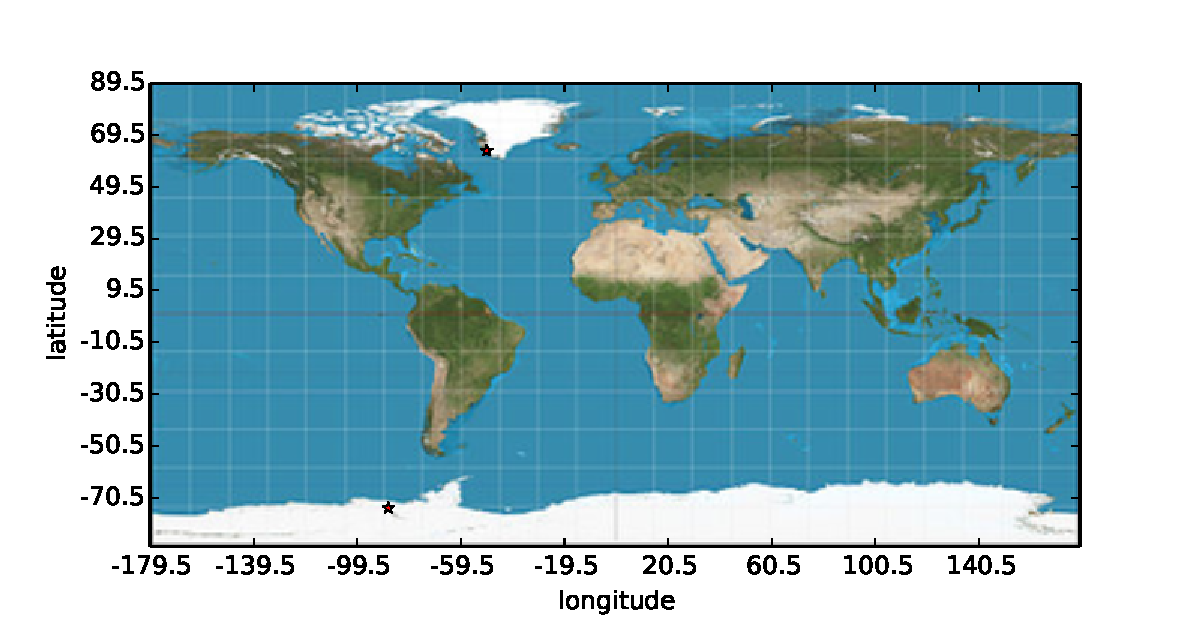
\includegraphics[height=6cm]{figures/ols-selected-map}
	\caption{The two selected locations, marked with a red star}
\end{figure}

\paragraph{Greenland}

At the west coast of Greenland is a strong period trend, caused by the the ice melting over the summer and reappearing over the winter. This trend is seen in Figure \ref{fig:ols-selected-0-fit}. In order to estimate the velocity and acceleration of the EWH, there isn't caused by some season, it's important that the periodc trend is caught by the $\sin(\cdot)$ and $\cos(\cdot)$ terms in OLS regression.
\begin{figure}[H]
	\centering
	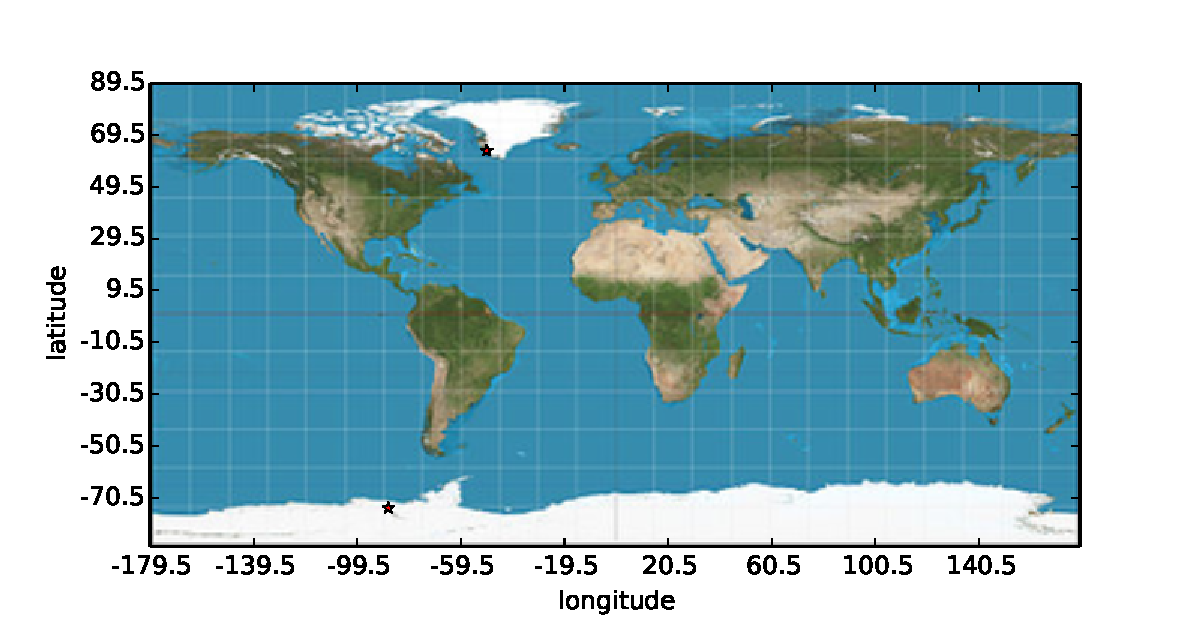
\includegraphics[width=\textwidth]{figures/ols-selected-0-fit}
	\caption{Messurements are blue, the OLS fit is red.}
	\label{fig:ols-selected-0-fit}
\end{figure}
 
From Figure \ref{fig:ols-selected-0-fit} it's seen that the period trend is caught by the model, however for some seasons (particular between 2008 and 2010) the fit is not very good. This is even more clear when looking at the residuals (Figure \ref{fig:ols-selected-0-residual}). From this it's clear that the residuals are far from white noise, which was one of the OLS assumptions.
\begin{figure}[H]
	\centering
	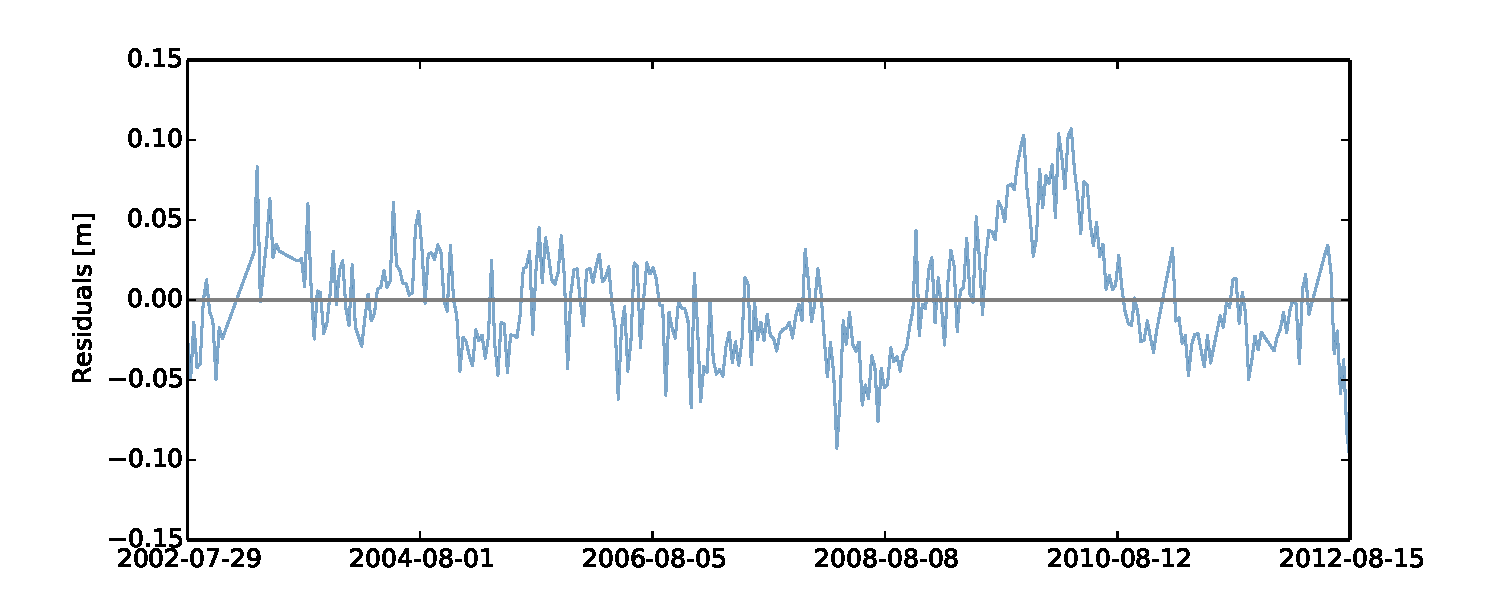
\includegraphics[width=\textwidth]{figures/ols-selected-0-residual}
	\caption{The OLS residuals are blue.}
	\label{fig:ols-selected-0-residual}
\end{figure}

Besides the yearly season, there is when looking at the estimated OLS coefficients (Table \ref{table:ols-selected-0-paramters}) also a half yearly season. Though strangely enough it isn't very visible on the OLS fit (Figure \ref{fig:ols-selected-0-fit}). The remaining seasons are with 95\% confidence not significantly different from zero and for the purpose of getting a better estimate, it might be worth iteratively removing these terms.
\begin{table}[H]
\centering
\centerline{\begin{tabular}{r|rr}
\hline
 name                                & estimate              & p-value   \\
\hline
 $intercept (1)$                     & $-1.77 \cdot e^{-01}$ & $0.000$   \\
 $vel. (t)$                          & $-2.24 \cdot e^{-04}$ & $0.000$   \\
 $acc. (0.5 \cdot t^2)$              & $-8.27 \cdot e^{-08}$ & $0.000$   \\
 $\cos(\sfrac{2\pi}{365.2} \cdot t)$ & $-1.35 \cdot e^{-02}$ & $0.000$   \\
 $\sin(\sfrac{2\pi}{365.2} \cdot t)$ & $-8.28 \cdot e^{-02}$ & $0.000$   \\
 $\cos(\sfrac{2\pi}{182.6} \cdot t)$ & $-5.86 \cdot e^{-03}$ & $0.045$   \\
 $\sin(\sfrac{2\pi}{182.6} \cdot t)$ & $-1.41 \cdot e^{-02}$ & $0.000$   \\
 $\cos(\sfrac{2\pi}{121.7} \cdot t)$ & $-5.01 \cdot e^{-03}$ & $0.089$   \\
 $\sin(\sfrac{2\pi}{121.7} \cdot t)$ & $-5.69 \cdot e^{-03}$ & $0.053$   \\
 $\cos(\sfrac{2\pi}{91.3} \cdot t)$  & $-5.49 \cdot e^{-03}$ & $0.060$   \\
 $\sin(\sfrac{2\pi}{91.3} \cdot t)$  & $-1.66 \cdot e^{-03}$ & $0.573$   \\
 $\cos(\sfrac{2\pi}{73.0} \cdot t)$  & $-2.19 \cdot e^{-03}$ & $0.455$   \\
 $\sin(\sfrac{2\pi}{73.0} \cdot t)$  & $-1.93 \cdot e^{-03}$ & $0.511$   \\
 $\cos(\sfrac{2\pi}{60.9} \cdot t)$  & $4.29 \cdot e^{-04}$  & $0.883$   \\
 $\sin(\sfrac{2\pi}{60.9} \cdot t)$  & $1.43 \cdot e^{-03}$  & $0.627$   \\
 $\cos(\sfrac{2\pi}{52.2} \cdot t)$  & $9.55 \cdot e^{-04}$  & $0.744$   \\
 $\sin(\sfrac{2\pi}{52.2} \cdot t)$  & $1.09 \cdot e^{-04}$  & $0.970$   \\
 $\cos(\sfrac{2\pi}{45.7} \cdot t)$  & $-3.08 \cdot e^{-04}$ & $0.916$   \\
 $\sin(\sfrac{2\pi}{45.7} \cdot t)$  & $-2.37 \cdot e^{-04}$ & $0.935$   \\
 $\cos(\sfrac{2\pi}{40.6} \cdot t)$  & $-2.02 \cdot e^{-03}$ & $0.491$   \\
\hline
\end{tabular}\hspace{1cm}\begin{tabular}{r|rr}
\hline
 name                               & estimate              & p-value   \\
\hline
 $\sin(\sfrac{2\pi}{40.6} \cdot t)$ & $8.48 \cdot e^{-04}$  & $0.772$   \\
 $\cos(\sfrac{2\pi}{36.5} \cdot t)$ & $1.54 \cdot e^{-03}$  & $0.599$   \\
 $\sin(\sfrac{2\pi}{36.5} \cdot t)$ & $-5.77 \cdot e^{-04}$ & $0.843$   \\
 $\cos(\sfrac{2\pi}{33.2} \cdot t)$ & $-5.95 \cdot e^{-04}$ & $0.839$   \\
 $\sin(\sfrac{2\pi}{33.2} \cdot t)$ & $-1.47 \cdot e^{-03}$ & $0.615$   \\
 $\cos(\sfrac{2\pi}{30.4} \cdot t)$ & $1.78 \cdot e^{-04}$  & $0.952$   \\
 $\sin(\sfrac{2\pi}{30.4} \cdot t)$ & $5.37 \cdot e^{-04}$  & $0.854$   \\
 $\cos(\sfrac{2\pi}{28.1} \cdot t)$ & $2.57 \cdot e^{-03}$  & $0.383$   \\
 $\sin(\sfrac{2\pi}{28.1} \cdot t)$ & $-6.35 \cdot e^{-04}$ & $0.827$   \\
 $\cos(\sfrac{2\pi}{26.1} \cdot t)$ & $3.16 \cdot e^{-04}$  & $0.914$   \\
 $\sin(\sfrac{2\pi}{26.1} \cdot t)$ & $-2.99 \cdot e^{-04}$ & $0.919$   \\
 $\cos(\sfrac{2\pi}{24.3} \cdot t)$ & $-7.23 \cdot e^{-04}$ & $0.804$   \\
 $\sin(\sfrac{2\pi}{24.3} \cdot t)$ & $3.33 \cdot e^{-04}$  & $0.910$   \\
 $\cos(\sfrac{2\pi}{22.8} \cdot t)$ & $-8.07 \cdot e^{-04}$ & $0.785$   \\
 $\sin(\sfrac{2\pi}{22.8} \cdot t)$ & $-6.93 \cdot e^{-04}$ & $0.811$   \\
 $\cos(\sfrac{2\pi}{21.5} \cdot t)$ & $-1.26 \cdot e^{-03}$ & $0.665$   \\
 $\sin(\sfrac{2\pi}{21.5} \cdot t)$ & $-7.28 \cdot e^{-04}$ & $0.803$   \\
 $\cos(\sfrac{2\pi}{20.3} \cdot t)$ & $-4.93 \cdot e^{-04}$ & $0.864$   \\
 $\sin(\sfrac{2\pi}{20.3} \cdot t)$ & $-9.94 \cdot e^{-06}$ & $0.997$   \\
                                    &                       &           \\
\hline
\end{tabular}}
\caption{Parameter esimates $\hat{\beta}$ and their p-values. }
\label{table:ols-selected-0-paramters}
\end{table}

\paragraph{South Pole}

Just like with Greenland there is a clear drop in mass as seen in Figure \ref{fig:ols-selected-1-fit}. However interestingly enough there is no seasonal trend or at least it's not very strong. Also the existence of high frequency terms on the OLS regression, is more apparent. Though from the actual data it don't look like such period trend exists. This suggests that to many frequency terms have been used, thus causing some overfitting.
\begin{figure}[H]
	\centering
	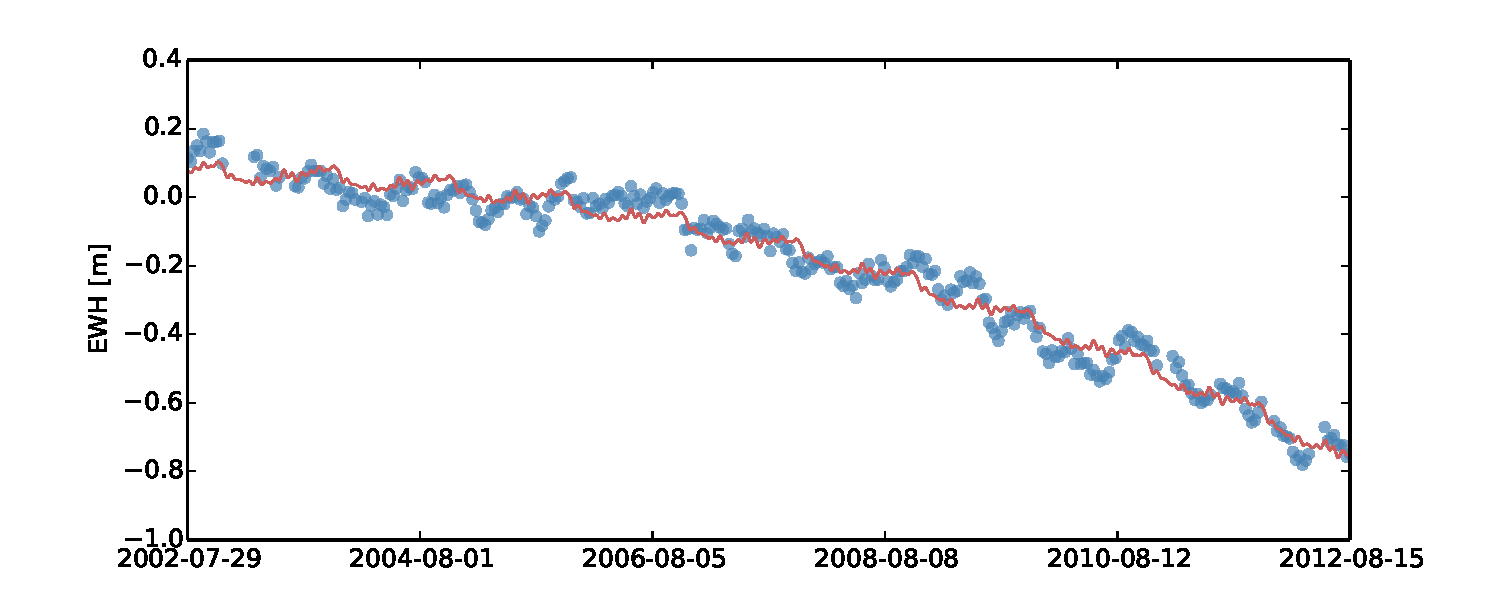
\includegraphics[width=\textwidth]{figures/ols-selected-1-fit}
	\caption{Messurements are blue, the OLS fit is red.}
	\label{fig:ols-selected-1-fit}
\end{figure}

When looking at the residuals in Figure \ref{fig:ols-selected-1-residual}, it's again clear that the residuals are far from being white noise. There also seams to be some periodic trend in the residuals, though the beginning and the end of these seasons is quite hard to make out. 

\begin{figure}[H]
	\centering
	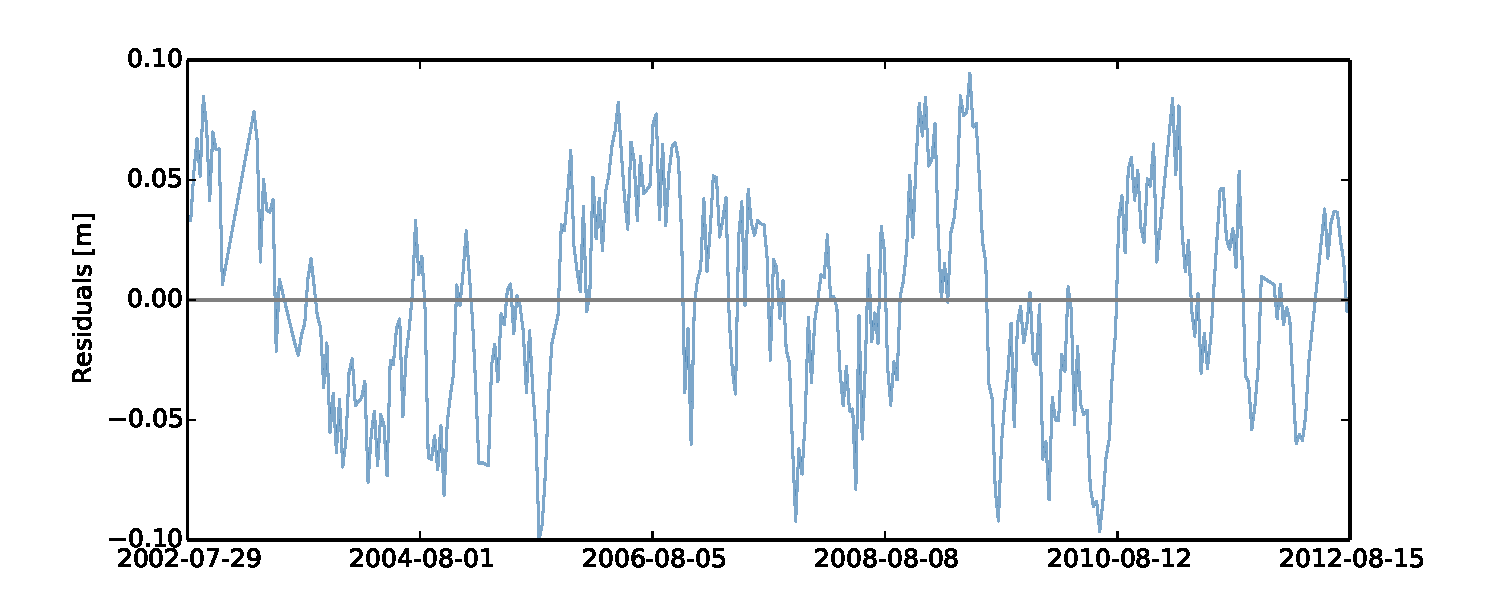
\includegraphics[width=\textwidth]{figures/ols-selected-1-residual}
	\caption{The OLS residuals are blue.}
	\label{fig:ols-selected-1-residual}
\end{figure}

Just as with Greenland many of the OLS terms are with 95\% confidence not significantly different from zero. Interestingly enough there is a yearly season when looking at Table \ref{table:ols-selected-1-paramters}, though it's very hard to make out from the OLS fit in Figure \ref{fig:ols-selected-1-fit}.

\begin{table}[H]
\centering
\centerline{\begin{tabular}{r|rr}
\hline
 name                           & estimate               & p-value   \\
\hline
 $intercept (1)$                & $-1.38 \cdot 10^{-01}$ & $0.000$   \\
 $vel. (t)$                     & $-2.26 \cdot 10^{-04}$ & $0.000$   \\
 $acc. (0.5 \cdot t^2)$         & $-1.24 \cdot 10^{-07}$ & $0.000$   \\
 $\cos(1 \cdot \omega \cdot t)$ & $1.69 \cdot 10^{-02}$  & $0.000$   \\
 $\sin(1 \cdot \omega \cdot t)$ & $1.42 \cdot 10^{-02}$  & $0.000$   \\
 $\cos(2 \cdot \omega \cdot t)$ & $-7.19 \cdot 10^{-03}$ & $0.046$   \\
 $\sin(2 \cdot \omega \cdot t)$ & $2.82 \cdot 10^{-03}$  & $0.440$   \\
 $\cos(3 \cdot \omega \cdot t)$ & $-4.36 \cdot 10^{-03}$ & $0.227$   \\
 $\sin(3 \cdot \omega \cdot t)$ & $-1.23 \cdot 10^{-03}$ & $0.732$   \\
 $\cos(4 \cdot \omega \cdot t)$ & $1.78 \cdot 10^{-03}$  & $0.619$   \\
 $\sin(4 \cdot \omega \cdot t)$ & $2.81 \cdot 10^{-03}$  & $0.437$   \\
 $\cos(5 \cdot \omega \cdot t)$ & $2.45 \cdot 10^{-03}$  & $0.496$   \\
 $\sin(5 \cdot \omega \cdot t)$ & $2.53 \cdot 10^{-03}$  & $0.484$   \\
 $\cos(6 \cdot \omega \cdot t)$ & $-1.60 \cdot 10^{-03}$ & $0.654$   \\
 $\sin(6 \cdot \omega \cdot t)$ & $-8.66 \cdot 10^{-04}$ & $0.811$   \\
 $\cos(7 \cdot \omega \cdot t)$ & $8.95 \cdot 10^{-04}$  & $0.803$   \\
 $\sin(7 \cdot \omega \cdot t)$ & $-3.27 \cdot 10^{-03}$ & $0.364$   \\
 $\cos(8 \cdot \omega \cdot t)$ & $1.62 \cdot 10^{-03}$  & $0.652$   \\
 $\sin(8 \cdot \omega \cdot t)$ & $-1.51 \cdot 10^{-03}$ & $0.674$   \\
 $\cos(9 \cdot \omega \cdot t)$ & $3.76 \cdot 10^{-04}$  & $0.917$   \\
\hline
\end{tabular}\hspace{1cm}\begin{tabular}{r|rr}
\hline
 name                            & estimate               & p-value   \\
\hline
 $\sin(9 \cdot \omega \cdot t)$  & $2.05 \cdot 10^{-03}$  & $0.568$   \\
 $\cos(10 \cdot \omega \cdot t)$ & $-4.54 \cdot 10^{-04}$ & $0.900$   \\
 $\sin(10 \cdot \omega \cdot t)$ & $-1.26 \cdot 10^{-03}$ & $0.726$   \\
 $\cos(11 \cdot \omega \cdot t)$ & $-1.21 \cdot 10^{-04}$ & $0.973$   \\
 $\sin(11 \cdot \omega \cdot t)$ & $-1.07 \cdot 10^{-03}$ & $0.766$   \\
 $\cos(12 \cdot \omega \cdot t)$ & $-1.20 \cdot 10^{-03}$ & $0.740$   \\
 $\sin(12 \cdot \omega \cdot t)$ & $-8.20 \cdot 10^{-04}$ & $0.819$   \\
 $\cos(13 \cdot \omega \cdot t)$ & $-5.73 \cdot 10^{-03}$ & $0.114$   \\
 $\sin(13 \cdot \omega \cdot t)$ & $-8.50 \cdot 10^{-04}$ & $0.812$   \\
 $\cos(14 \cdot \omega \cdot t)$ & $-6.55 \cdot 10^{-04}$ & $0.855$   \\
 $\sin(14 \cdot \omega \cdot t)$ & $2.25 \cdot 10^{-03}$  & $0.533$   \\
 $\cos(15 \cdot \omega \cdot t)$ & $-4.32 \cdot 10^{-04}$ & $0.904$   \\
 $\sin(15 \cdot \omega \cdot t)$ & $3.05 \cdot 10^{-04}$  & $0.933$   \\
 $\cos(16 \cdot \omega \cdot t)$ & $3.51 \cdot 10^{-04}$  & $0.923$   \\
 $\sin(16 \cdot \omega \cdot t)$ & $-3.73 \cdot 10^{-04}$ & $0.917$   \\
 $\cos(17 \cdot \omega \cdot t)$ & $1.22 \cdot 10^{-03}$  & $0.735$   \\
 $\sin(17 \cdot \omega \cdot t)$ & $-1.11 \cdot 10^{-03}$ & $0.758$   \\
 $\cos(18 \cdot \omega \cdot t)$ & $-1.92 \cdot 10^{-04}$ & $0.957$   \\
 $\sin(18 \cdot \omega \cdot t)$ & $7.18 \cdot 10^{-04}$  & $0.844$   \\
                                 &                        &           \\
\hline
\end{tabular}}
\caption{Parameter esimates $\hat{\beta}$ and their p-values. }
\label{table:ols-selected-1-paramters}
\end{table}
